\subsection{Spare matrix representation}

The first speed-up we look at utilises the \emph{sparseness} of the boundary matrix. To motivate, we consider a triangulation of $S^n$. Let $K$ be a simplicial complex consisting of the proper faces of some $(n+1)$-simplex and $\mathbb K$ be a maximal filtration of $K$ where we add the $0$-simplices, then the $1$-simplices, and so on. We note that there is $2^{n+2} - 2$ simplices. For $n = 2$, Figure \ref{fig:sparse-matrix-ex} shows a boundary matrix for $\mathbb K$ (recall that we are in $\mathbb F_2$, a blue square represents a 1 and a grey square represents a 0).

\begin{figure}
  \centering
  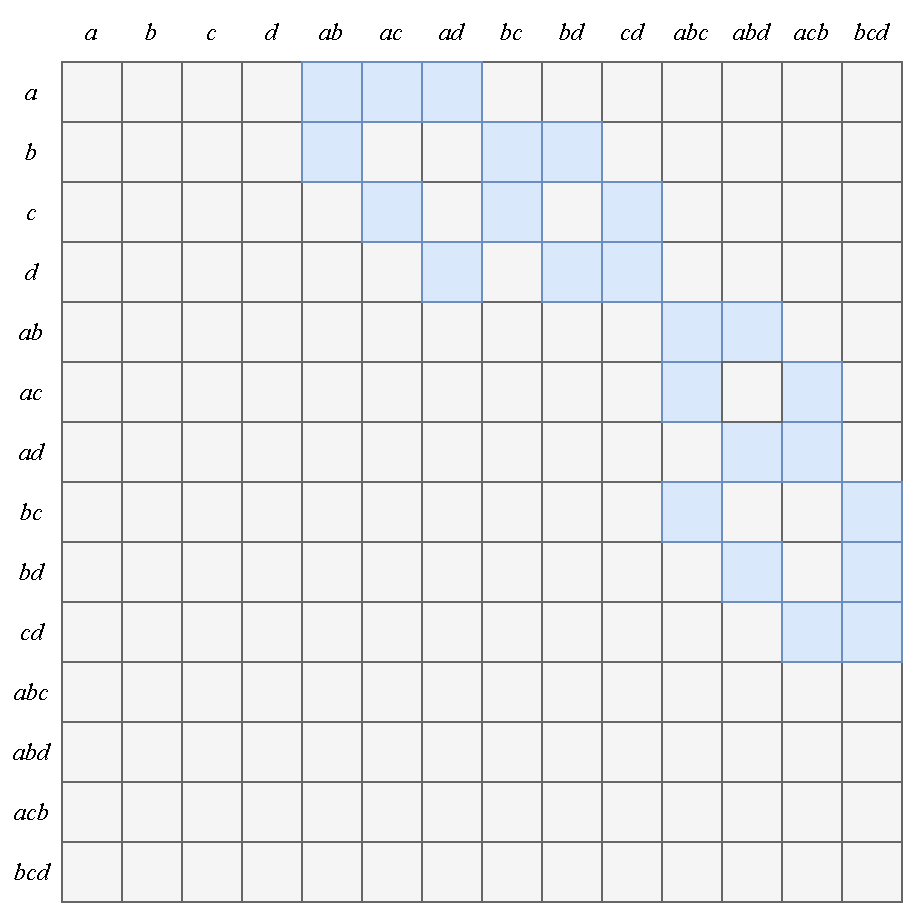
\includegraphics[width=0.7\textwidth]{content/4-comp-top/images/sparse-matrix-ex}
  \caption{A sparse boundary matrix for a filtration of a triangulation of $S^2$. A grey square represents a $0$ entry in the matrix, and a blue square represents a $1$.}
  \label{fig:sparse-matrix-ex}
\end{figure}

Figure \ref{fig:sparse-matrix-ex} shows a \emph{sparse matrix}; most of the entries are zero. Boundary matrices for general filtered simplicial complex are also sparse. Although most entries are 0, we are still storing each one: the standard algorithm stores a value for each $(i, j) \in (1, \ldots, n)^2$. There are many efficient methods for storing a sparse matrix, and most make use of assuming all entries are zero, then provide additional information for the non-zero entries. We will provide one such way of doing this, which is suited to our problem. 

\begin{figure}
  \centering
  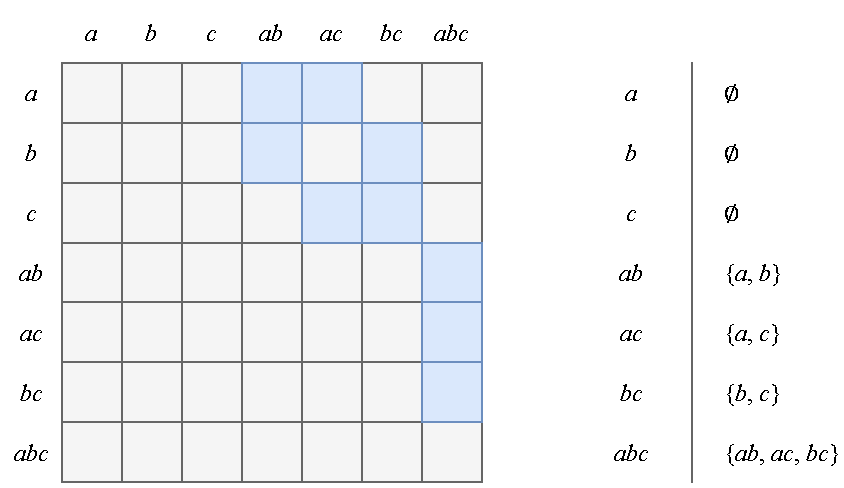
\includegraphics[width=0.9\textwidth]{content/4-comp-top/images/sparse-representation-ex}  
  \caption{On the left, the boundary matrix for the simplex ordering $(a, b, c, ab, ac, bc, abc)$. On the right, the sparse matrix representation. A grey square represents a $0$ entry in the matrix, and a blue square represents a $1$.}
  \label{fig:sparse-representation-ex}
\end{figure}

Let $A \in M_n(\mathbb F_2)$ be a matrix. For each column $j \in \{1, \ldots n\}$, we store a set (hash table), denoted $S_j$, such that $i \in S_j$ if and only if $A[i,j] = 1$. This allows constant time for many elementary operations (such as membership queries, insertion, and deletion) and constant space. Figure \ref{fig:sparse-representation-ex} shows an example of this representation. We further comment on the running time of operations with this data structure, specific to the reduction algorithm. For $i \in \{1, \ldots, n\}$, denote the number of non-zero entries in column $i$ by $m_i$, and we have $O(m_i) = O(d)$.

\begin{enumerate}
  \item Column operations: let $i, j \in \{1, \ldots, n\}$ . Then the time to add column $j$ to $i$ is $O(m_i + m_j)$. Given that we typically fix the dimensions to compute homology to, we can take this as constant (or as $O(d)$ for maximum dimension $d$).
  \item Retrieve the last non-zero entry in column: let $i \in \{1, \ldots, n\}$. Finding the last non-zero entry in $i$ is $O(m_i)$.
\end{enumerate}

As we are just modifying the underlying data structure, the algorithm does not change significantly and thus will not be repeated here. We refer to the standard algorithm with sparse matrix representation as \textsc{SS}. 

This analysis provides a convincing argument the effectiveness of this speed-up. To quantify this, an experiment was conducted in which measured the running time for both loading (that is, taking a filtration and computing its boundary matrix) and the matrix reduction for the standard triangulation of $S^n$ for $n \in \{1, \ldots, 9\}$. The running times can be seen in Figure \ref{fig:speedups-1v2-compute} and the loading running times can be seen in Figure \ref{fig:speedups-1v2-load}.

\begin{figure}
  \makebox[\textwidth][c]{
    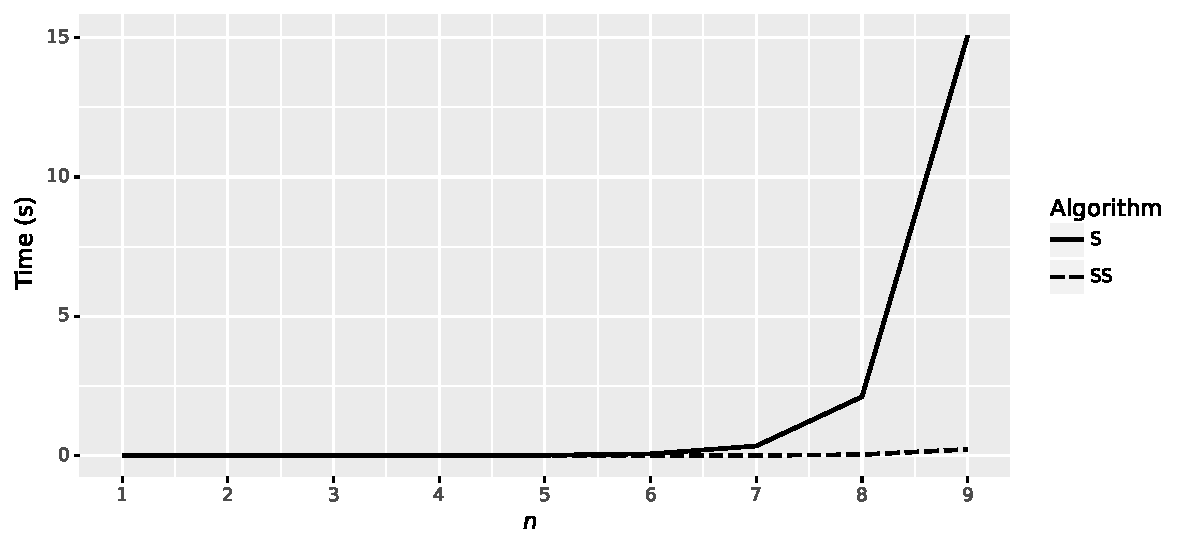
\includegraphics[width=1.2\textwidth]{content/4-comp-top/images/2-1v2-compute}
  }
  \caption{A plot of the running time of the \textsc{SS} algorithm versus the \textsc{S} algorithm for filtrations of triangulations of $S^n$.}
  \label{fig:speedups-1v2-compute}
\end{figure}

\begin{figure}
  \makebox[\textwidth][c]{
    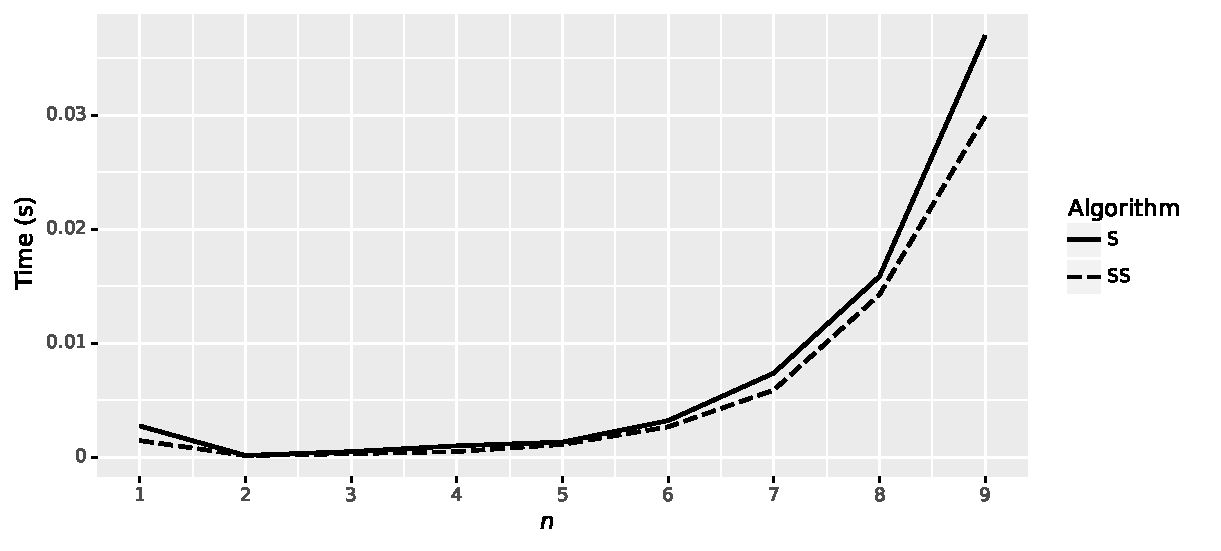
\includegraphics[width=1.2\textwidth]{content/4-comp-top/images/2-1v2-load}
  }
  \caption{A plot of the running time of the construction of the boundary matrix (loading time) using the standard matrix representation versus the sparse matrix representation, for filtrations of triangulations of $S^n$.}
  \label{fig:speedups-1v2-load}
\end{figure}

From this experiment, we see that the sparse matrix representation significantly decreases the time taken by the reduction; however, it does not decrease the loading time. This is to be expected as we still need to iterate over every the facets of every simplex; however, we note that this input serves as a worse case for loading time, so we would expect a large running time for loading compared to other inputs.

Another experiment was conducted using a Vietoris-Rips complex (with $\hat\varepsilon = 0.01$) constructed from point-cloud data sampled from a noisy unit circle (radius fluctuation $0.1$). Each algorithm was executed on a complex constructed from $n$ points, where $n \in \{100, 200, \ldots, 1500\}$. Figure \ref{fig:speedups-1v2-circ-compute} shows the running time of both of these algorithms, and it is clear that the sparse representation is still significantly faster.

\begin{figure}
  \makebox[\textwidth][c]{
    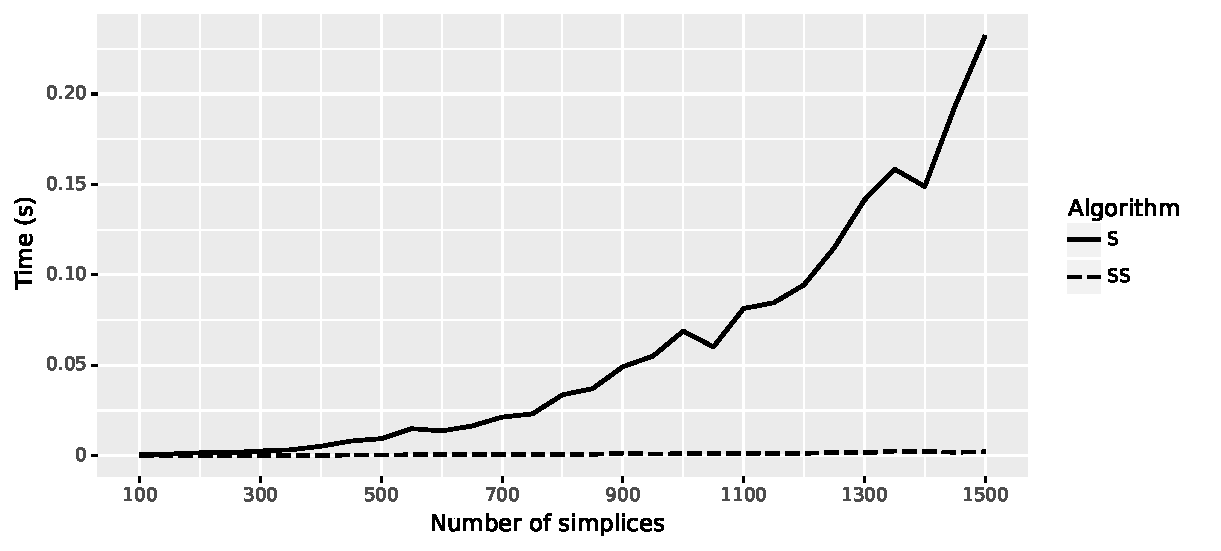
\includegraphics[width=1.2\textwidth]{content/4-comp-top/images/2-1v2-circ-compute}
  }
  \caption{A plot of the running time of the \textsc{SS} algorithm versus the \textsc{S} algorithm for Vietoris-Rips complexes constructed from noisy unit circle data.}
  \label{fig:speedups-1v2-circ-compute}
\end{figure}

We note that there are other data structure choices that could be made instead of hash tables. For example, for each column we may instead store some sorted data structure. If we use a list sorted by index then we can retrieve the lowest non-zero entry in constant time, but we have $O(n)$ time for insertion, deletion, and membership queries. Binary search trees could also be used, which would allow us to find the lowest non-zero entry in $O(\log n)$ average time, as well as $O(\log n)$ average time for insertion, deletion, and membership queries. Utilising self-balancing tree structures (such as B-trees), the worst-case time can also be brought down to $O(\log n)$.

We highlight the use of various data structures for storing a boundary matrix to be a topic of further research.
